\documentclass[12pt]{article}
\usepackage[a4paper]{geometry}
\usepackage{fullpage}
\usepackage[UKenglish]{babel}
\usepackage[utf8]{inputenc}
\usepackage{graphics,epsfig}
\usepackage{tabularx,colortbl}
\usepackage{url}
\usepackage{lastpage}
\usepackage{fancyhdr}
\usepackage[parfill]{parskip}
\usepackage{wrapfig}
\usepackage{minted}
\usepackage{hyperref}
\hypersetup{
    colorlinks=true,
    linkcolor=blue,
    filecolor=magenta,      
    urlcolor=cyan
    }
\pagestyle{fancy} 
\renewcommand{\headrulewidth}{0pt}
\fancyhf{}
\fancypagestyle{plain}{%
  \renewcommand{\headrulewidth}{0pt}%
  \fancyhf{}%
  \fancyfoot[C]{\footnotesize \thepage\ of \pageref{LastPage}}%
}
\fancyfoot[C]{\footnotesize  \thepage\ of \pageref{LastPage}}

\usepackage{listings}

\title{
\includegraphics[width=0.8\textwidth]{uia-logo.png}~\\[1cm]
Scala Project Report}

\date{IKT212\\
24.09.2021}
\author{Group 13\\
Anders Lauvrak Espenes, Andreas Martinius Feragen\\
andersle, andrmf18}

\begin{document}
\maketitle


\section*{Abstract}
This document, is a report for the light-up solver we made as part of the IKT212 course. The problem was to use the scala programming language and a function paradigm to create a solver for a puzzle called light-up/akari. Our solver uses a combination of a simple trivial solver and backtracking to solve the puzzle. Lastly the document also details on the planning of the project and reflection around the assignment.


\newpage


\section{Introduction}
\subsection{Akari}
In this assignment, we are tasked with creating a piece of software that solves a light-up puzzle, also known as Akari. A light-up puzzle contains a grid of $NxM$ size, with randomly placed walls/black squares on the board. The walls may hold nothing or a number between $0..4$. The goal of the game is to light up all the white tiles. The player place lights on the board, lighting up white tiles on the horizontal and vertical axis of the placed light. If there is a wall on the same axis as a light, then only the white tiles between the light and the wall are lit up. The rules are that no light shall shine on another light, and every numbered wall must have the numbered amount of light in its adjacent tiles. Each puzzle has exactly one solution.

\subsection{Assignment requirements}
A requirement for this assignment is to use the scala programming language and use a functional approach. The assignment is tested through bamboos automated testing system. The code is compiled and ran with two files given as arguments. The first argument contains file path to the unsolved board, and the last argument will be the file path where we will write the solved board too. We follow the Plan Execute Reflect methodology, which this report is part of the reflection.


\subsection{Report structure} 
This report describes how our solution solves a light-up puzzle and why we chose this method. Then we tell how we implemented our solution, how we approached the problem to write the code. The correctness section describes why our solution works, why it finds a solution and the methods we used to ensure the code works as intended. The plan and reflection section describes our project planning and reflection of the assignment.



\section{Solution}
% Describe your solution including the following elements. Use code pieces where appropriate.
Our solution uses heuristics and backtracking to solve the puzzles. Backtracking is an algorithm that solves constraint satisfaction problems, which means for light-up each white tile is a state, and the rules of the game are the constraints. Although backtracking is better than a brute force approach, it will still make guesses. This means that the larger the board, the more possible paths the algorithm can take. Therefore, it is essential to narrow down the possibilities with heuristics before starting the algorithm. This is done by using the rules to our advantage and knowingly placing lights at tiles that are guaranteed to have one there.


\subsection{Coding Strategy}
\label{coding strat}
% Gå over hvordan vi har/hadde lyst til å skrive
% Gå over hvordan vi tenke programmet skulle være satt opp, "arkitekturen"
% Gå over/ vise hvordan vi representere spillet og løsning


For this project, our strategy was to use unit testing. It didn't necessarily involve using test driven development to write our code because we wanted to use unit tests where it made sense or needed. Doing this, we had mainly two reasons, correctness and decoupling. We want to confidently change or refactor code, knowing our program didn't break under certain conditions. This would help us save time, either from debugging later or doing lots of manual testing. Writing our code with testing in mind will most likely result in less coupling in our code. This is something that we want, again to make it easier to change and refactor code. Writing code with low coupling is also a good thing most of the time.

Making our code with low coupling would allow us to easier change our code later. We don't plan on writing the most functional or best code at the start. We consider it is more important to have a working solution. This doesn't mean we plan to write bad and non-functional code, but rather that we move on to the next task when encountering problems where we can't think of a good or functional solution. This means that some of the code won't be optimal, but we can thru the end of the project delegate time to solve some of these issues or focus our time on parts of code that we are less happy with, like performance. Hopefully, we can write decoupled code with high cohesion. Then refactoring at the end won't be as much of a challenge.


\subsection{Program structure}
% Choose a simple way to represent the puzzle.
% unsure if there is a faster or better method, but we valued a representation that made development easier

The program is structured into two main objects $PuzzleSolver$ and $solver$, where the former is the main object and entry point of the program. There are also several supporting objects, such as $PuzzleReaderWriter$ which reads and writes to files; a package object $types$ which hold useful variables and types, lastly a $Puzzle$ class which holds a puzzle with meta information and the solve and unsolved board itself.

The $PuzzleSolver$ program functions as the controller and invokes the other classes and objects in the order required to solve the puzzle. It starts by taking the first argument, a file path containing a puzzle, and uses $PuzzleReaderWriter$ to read the puzzle. Then it invokes its solve method, where we first attempt heuristics to place lights on the puzzle board, then find possible candidates and lastly solve the puzzle by backtracking. Once a puzzle has been solved, it takes the second argument, a file path, and writes the solved board to the that file.

For representing the board we decided too simply store it as a 2d list of chars. This was made into a type called Matrix and the different chars had there corresponding variable so we could avoid hard coding the characters. We also created a simple class the represented a single position with a row and column. The reason we choose to represent to board as a 2d list was mostly do to simplicity. We understand that there is most likely is a faster or better method for representing the board; However we value being able to work with a familiar datatype and the ability to easily visualise the board when developing or debugging.



\subsubsection{Trivial solver}\label{trivialsolver}
\begin{wrapfigure}[24]{R}{0.4\textwidth}
    \begin{center}
    \centering
    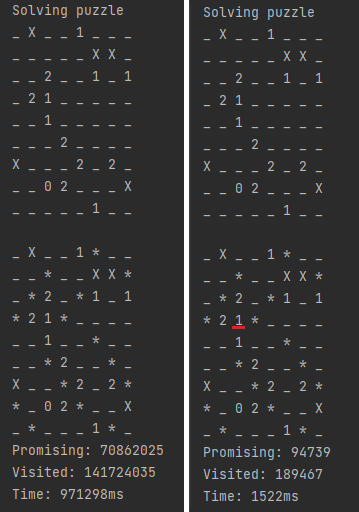
\includegraphics[scale=0.7]{doc/deterministic_vs_backtracking_only_hard.png}
    \caption{Difference when solving with and without placing using the trivial solver before backtracking}
    \label{fig:det_vs_back}
    \end{center}
\end{wrapfigure}


In Akari there are certain situations where we can for certain know the placement of some light. There are multiple of these tricks, but we have only implemented one which is the easiest and possibly most effective. That is looking at all the numbers on the board and placing lights where the amount of valid light positions are equals to the number. So when we talk about our trivial solver, this is what we refer to.

We have implemented this with a recursive function that first find all the number with there positions on the board. It then sort them from highest to lowest. We also filter out number tiles that already have the correct amount of lights around them. This allows us to only check the interesting positions. 

To determine if there if we should place lights around a number we get the positions to the adjacent empty tiles. This is done with the $check\_adjacent$ function. To get the empty adjacent tiles that is valid to place a light on we give the function $check\_placement$ as its condition argument. This is important as we are only interested in the tiles that we can legally place a light. To determine if we can place lights in the empty tiles we need to know how many adjacent lights the number tile has as well. If the sum of adjacent lights and empty tiles is equals to the number it mean we can place lights in the adjacent empty tiles. Looking at figure \ref{fig:det_vs_back} we can see that the marked 1 wall is the only number wall which we can place a light beside at first. Since the board has been changed we call the function again. With this one light placed we can now see this effects the 2 wall above. Since now one of its tiles is no longer a valid position. This means that there are only two valid adjacent tiles meaning we can place lights there. This again has an effect on the 1 at the top of the board. When the function has not been able to place any light, it returns it latest board.


We can see in figure \ref{fig:det_vs_back} the effect of this trivial solver. This example is on an somewhat difficult board and it shows the importance of using the trivial solver. The trivial solver only manages to place four lights, however its makes the board go from almost unsolvable\footnote{ 16 minuets is not unsolvable, but it is an unreasonable time to use on a board of this size } to being solved in under 2 seconds. This shows just how effective it is ti narrow the search space for the backtracker.


\newpage

\subsubsection{Backtracking}\label{backtracking}
\begin{wrapfigure}[13]{R}{0.4\textwidth}
\begin{center}
    \centering
    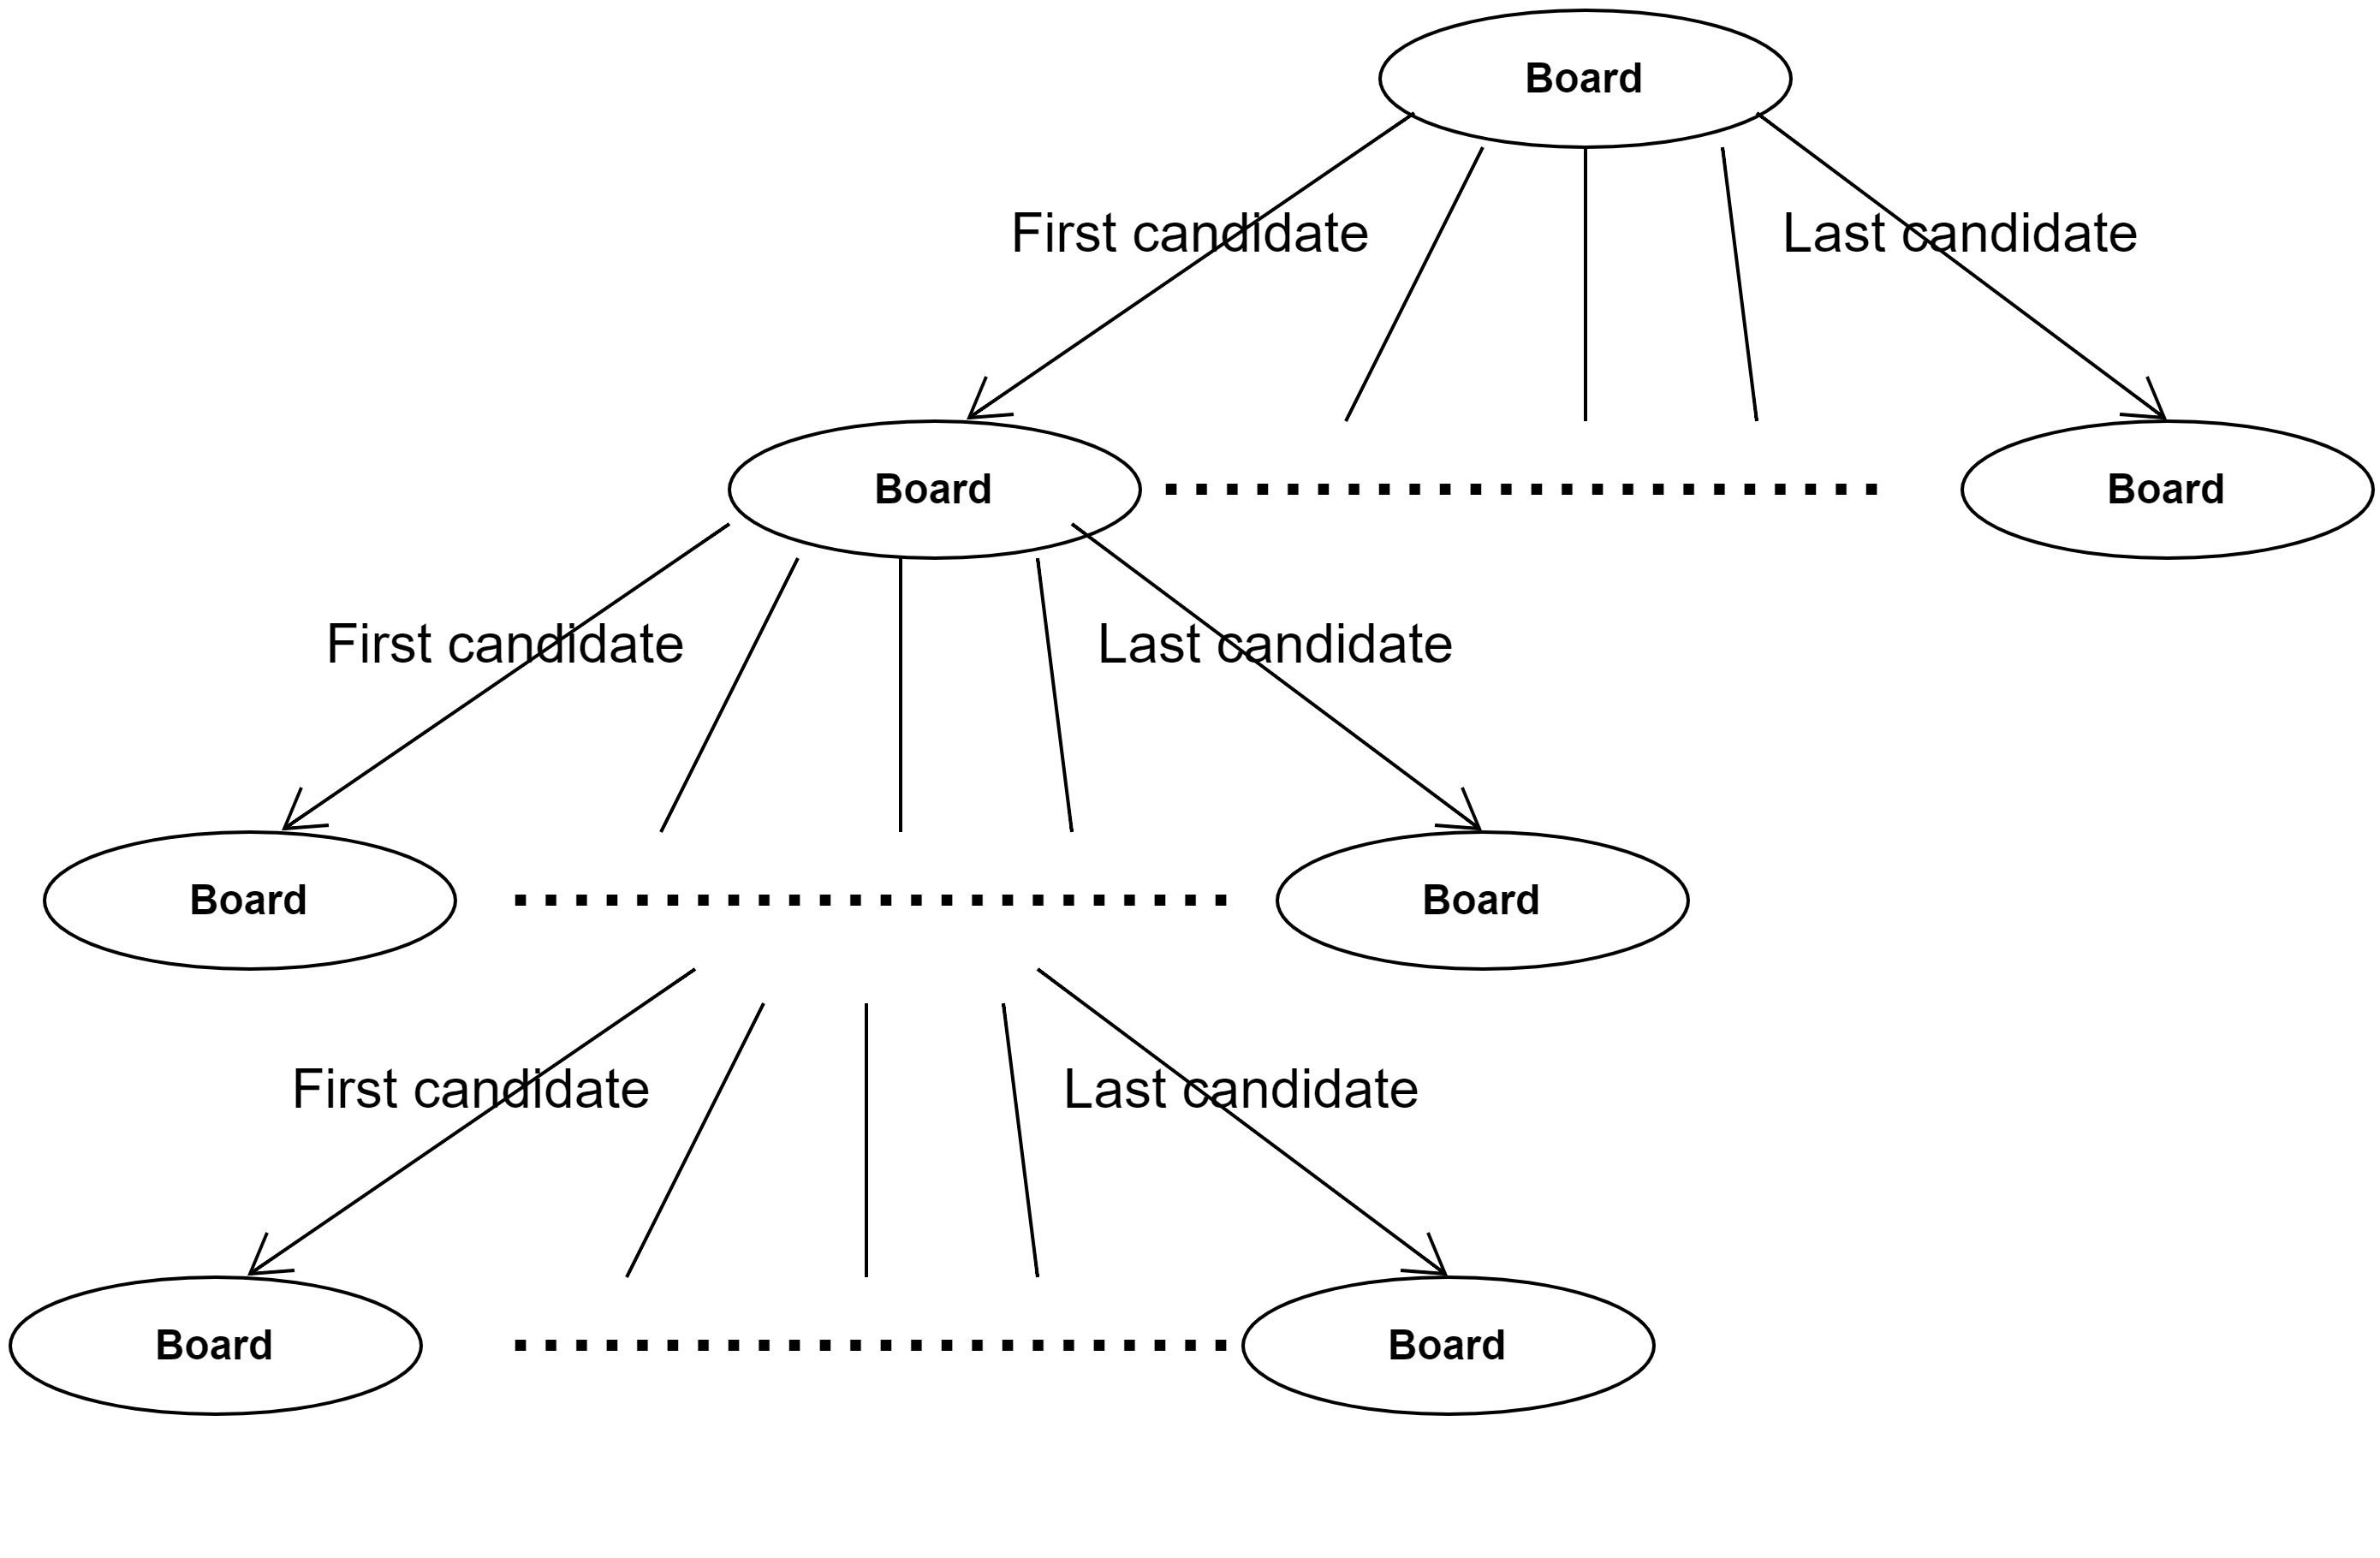
\includegraphics[width=0.4\textwidth]{doc/backtracking_tree.png}
    \caption{Shows the conceptual tree of the backtracking algorithm}
    \label{fig:tree}
    \end{center}
\end{wrapfigure}


Backtracking works by enumerating a set of selected candidates, trying out each candidate, and upon success, the next candidate is tried out recursively until all constraints are satisfied. A candidate makes a conceptual path between states of the board, each changed board is a node, and the set of nodes makes up a conceptual tree, with the recursive traversal being depth-first.


In our light-up puzzle, any white tile is considered a candidate for placement of light. There are two rules mentioned earlier that eliminate tiles as candidates. A white tile is not considered a candidate if there is a light in its column or row with no walls between them, or it is adjacent to a numbered wall, and there are already several lights placed adjacent to the wall equal to the number. The former is accomplished by the function $filter\_litup$ which takes in a board, a list of tile positions and the position of the light. The function will check if any tiles are on the same column or row as the given light and if there are no walls between them. To check if there are any walls between two positions the function: $check\_wall\_between\_tiles$ is used. It will take a board and two positions, and checks if any walls on the board are between the two positions.


The backtracking itself works through a recursive loop, where each invoke will attempt to place a light on a candidate tile on the board. If successful the function will filter out the newly lit up candidates and calls itself with the updated board and filtered candidates. It will attempt to place down a light on the next candidate until it solves the board, or no solution is found. No solution is found when there are no more candidates, and the board does not fulfil the requirements. At this point, the algorithm will return None and go back to a previous board state and call itself again, but instead of placing a light, the candidate position is removed. 

\subsubsection{Check Adjacent}
\label{check_adjacent}
Writing functional allowed us to make very generic functions. In our solution we needed to check the adjacent tiles of a position in a lot of cases. To do this we use the function $check\_adjacent$. This function takes another function with the signature $(Matrix, Position) => Boolean$ and returns a list of all the positions where this is true. The only function that is directly passed to $check\_adjacent$ is $check\_placement$, however with a helper function we can pass other functions to $check\_adjacent$ as well. This function, $char\_to\_board\_pos$ allows us to curry inn a function with the signature $Char => Boolean$ and get a function with $(Matrix, Position) => Boolean$ in return. This allows us to use the $check\_tile\_if\_$ functions with $check\_adjacent$. This can be seen in use in listing \ref{lst:check_adj} from which is from the $place\_light$ function.

\pagebreak
\begin{lstlisting}[language={Java}, basicstyle=\ttfamily\tiny, label={lst:check_adj}, caption={Code from place\_light function}]
if (check_adjacent(board, pos, char_to_board_pos(_: Matrix, _: Position, check_tile_if_num)).exists(num => {
  get_number_of_lights_around_number(board, num) >= board(num.row)(num.col).asDigit})) {
  return None
} else if (check_placement(board, pos))
  return Option(board.updated(pos.row, board(pos.row).updated(pos.col, Light)))
else
  return None
\end{lstlisting}


\section{Correctness}
% Følger krav om logisk/funksjonell programering bruker nesten et pipe and filter pattern, hver funksjon endrer bare på lokale variabler, og returnerer noe annet. Har ingen funksjoner som ikke er deterministiske. Eneste side effekts vi har er read and write?

As stated in \ref{coding strat} we wanted to use unit testing in this program. This is our staple source of correctness when making sure the program works and produces a correct solution. For most of the functions created, one or more unit tests were also created to check if the logic was correct. As we were required to program with a functional approach, we ended up using a pipe and filter pattern, where each function is self-contained without any side effects. Unit tests are great for these functions, as each function should be deterministic and produce the same result for the same input. So as long as the logic of each function is correct, without any oversights mind you, then chaining them together later should be logical and produce the desired result. 

% Vi passer på å ikke ha mutable variabler, OG om vi har det er det contained til enkelt funkjson
% Løser alle validate testene på bamboo, klarer brett opp til en viss størrelse, brett med flere vegger er vanskeligere for vår løsning, fordi ... Forklare hvorfor brett av størrelse NxM ikke kan løses med vår løsning.
% Åpne brett lettere, brett med flere vegger en empty tiles også lett, ja siden da kan trivial solver mest sannsynelig gjøre mye.
% Brett med 

\label{plan and ref}
\begin{wrapfigure}[17]{R}{0.3\textwidth}
\begin{center}
    \centering
    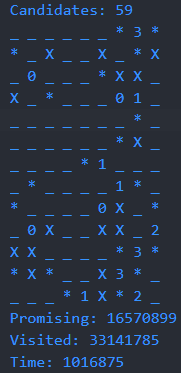
\includegraphics[width=0.2\textwidth]{doc/59Candidates.png}
    \caption{A solved board that starts with 59 candidates}
    \label{fig:9x13Solved}
\end{center}
\end{wrapfigure}

The efficiency of our solution depends on how many candidates the backtracking algorithm have to attempt. This means that how many candidates we start with and how fast they are eliminated, determines how quickly the solver finds a solution. As our trivial solver places down lights, as mentioned in \ref{trivialsolver}, how many lights and how many white tiles have lit up will have substantial effects on the speed of the solver. In figure \ref{fig:det_vs_back} we see how large of a difference the trivial solver makes. The solver without heuristics starts backtracking with 51 candidates, while with heuristics, the backtracking start with 31 candidates. The layout of the board also determines how quickly candidates are eliminated. A board with long paths without any walls allows for fewer lights to illuminate more tiles. An example we found of this is in figure \ref{fig:9x13Solved}, where the backtracking starts with 59 candidates while still finding a solution. Normally boards with this many candidates are unsolvable with our solution. 

\newpage
\section{Plan and Reflection}
\label{plan and ref}
\begin{wrapfigure}[18]{R}{0.5\textwidth}
    \begin{center}
        \centering
        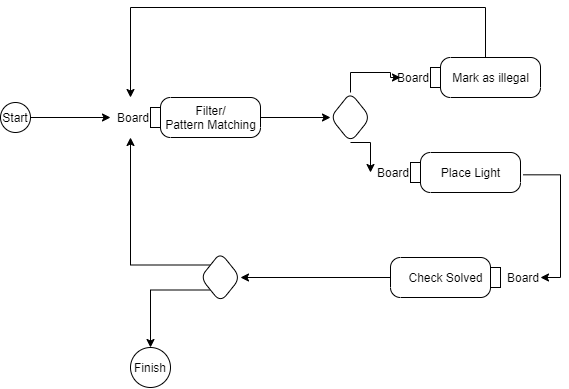
\includegraphics[width=0.6\textwidth]{doc/architecture.uml.drawio.png}
        \caption{Overview over how we wanted to solved the puzzle}
        \label{fig:architecture}
    \end{center}
\end{wrapfigure}


At the beginning of the project, we did not start solving the assignment straight away. We spent some time trying out scala and studying functional programming. We also researched how to tackle a puzzle-solving problem. Then we created a simple overarching plan, where we settled on using backtracking for solving the puzzle and then create some filters. The initial plan was specific regarding tasks we knew needed to be done such as creating a data structure, reading/writing files and checking if a board was solved. We also intentionally did not attempt to write the best and most functional code for these tasks, as we felt they were required to progress towards having a working solution, with plans to rewrite them later in the project. For those tasks we did not know the specifics, we created some general tasks, such as optimizing the algorithm, with some information gained from research. We also created a state diagram, see figure \ref{fig:architecture}, of how we tough the software would work.

Another part of our plan was to use GitHub\footnote{ We have made the repository public. It can be found \href{https://github.com/BANZZAAAIIII/IKT212_Akari}{her}}. This was to help us improve communication and collaboration. We wanted to actively use the issue feature to not only assign the tasks in \ref{our tasks} but also for other issues/things that emerge, like bugs. We also wanted to use GitHub to do code reviews so both of us are familiar with the code, to give feedback and fix possible issues. \newline


\subsection{Our Tasks}
\label{our tasks}
The tasks we created are composed of the title in bold followed by a description of the task, the estimated and actual time used. At the end there is a reflection on the task.

\textbf{Create data structure for representing the board}\\
Create data structure that hold data related needed for a single puzzle\\
Time Est: 30 min\\
Time used: 1h\\
Spent more time than necessary reading about scala data structures, list vs array etc. Ended up using a simple 2d array of chars. This was for conventions as it makes debugging easier.\\


\textbf{Read and write the board data structure}\\
Modify the example code to read puzzle(s) from file and save to puzzle data structure and write puzzle(s) data structure to file with correct format.\\
Time Est: 4h\\
Time used: 9h \\
Spent more time than necessary reading about scala, read/write in scala and with functional programming. Needs some refactoring, considers current code OK\\
Spent too much time learning Scala on this task, in retrospect I should have programmed other things with the language first for more efficient learning.\\


\textbf{Create function to determine if puzzle is solved}\\
Create a function to determine that the puzzle is solved. This function should check that all squares must be lit up and constraints for numbers valid\\
Time Est: 4h\\
Time used: 4h\\
This worked out relatively nicely as I could reuse functions, with some modification, to check for light from the previous task. That made that part of the problem easy to solve. Determining of correct amount lights are around a number wasn't difficult, but I was unable to create a “good” functional solution.\\


\textbf{Create a brute force algorithm to try and solve the puzzle}\\
Create an algorithm, possibly with backtracking, that can solve the puzzle.\\
Time Est: 6h\\
Time used: 14h\\
The backtracking algorithm proved to be more challenging than initially believed. At first, it was confusing how one would step over a candidate if it proved to not be able to hold a light. Another challenge was to wrap my head around how each board maintained its state when it was backtracked too. This required some extra attention and time to understand, as I was not familiar with scala at the time.


\textbf{Optimizing the algorithm}\\
Use game rules to solve certain part of the board by identifying areas where there is only one thing that can be done, eg placing lights around a 4 block, marking area around 0 invalid, ect\\
Time Est: 8h\\
Time used: 6h\\
As per the plan this was done somewhat late in the development and that made this a lot easier to solve. For identifying and placing lights at around numbers with only one solution. This was somewhat easy and quick to do as we could use functions already made. That was because we where trying to create useful functions general, so reusing them for this was trivial for this problem. \\
    

\textbf{Refactoring}\\
Identify areas in our code that can be improved for both readability and to make it more functional\\
Time Est: 6h\\
Time used: 7h\\
We felt that here wasn't that much to refactor due to our program being surprisingly short and being better at writing functional then expected. We nonetheless found things to refactor which was mostly older code and some that wasn't very readable. What we did refactor went very well.\\


\subsection{Reflection}
Generaly we felt that this project when very well. The puzzle was more approachable, then we first expected, when we first got used to 
% Generel følelse på hvordan vi følte projsketet gikk
% Følte det gikk bra
% Startet bra, dabbet litt av uke mellom 05/09 til 12/09, mye jobbing mellom 12/09 til 19/09
% Overankende greit å programmere i scala og funkjsonelt, føler det tvinger oss litt til å skrive brae/bedre funksjoner. Slik vi har skrevet programmet føler vi det er nokså naturlig å ikke ha side effects



\subsubsection{The Plan}
% Plan reflection notes:
% We forgot to track time spent on a task/issue
% We decided to use github issues instead of writing tasks in a google docs.
% A lot of discussion were either on chat messages in discord or orally, and where not written down (mistake)
% Did not recap and update a the initial general plan, rather did this orally and created issues as we decided a feature or change was needed.


We could improve on the planning. As shown in \ref{plan and ref} we created a general plan in the beginning. This plan stayed mostly the same throughout the project\footnote{ We somewhat disagree on if this is because the tasks where to general or big }. Our attention was more focused on the \href{https://github.com/BANZZAAAIIII/IKT212_Akari}{GitHub}  issues we created during the development. This made it harder to track our time as some issues were done unrelated to our tasks. For example, placing the light wasn't necessarily done as a part of any of the tasks. It was just done early in the project to get us started as. Placing the light should have been a task on its own. 

Even though it's difficult, creating a less general plan is an improvement we should try to make. Creating the tasks as issues in GitHub  might also be a good idea. Doing that would allow us to see when we see that every commit or branch has an issue/task assigned. Although if we are not careful or created a too general plan, we will just end up creating a plan as we go. This is something we have to keep in mind if we decide to do this next project. We should also have a more formal process for planing the next days, both in terms of creating new tasks/issues or what our work tasks will be. This was kinda done this project, however it was very informal and not everything that should have been recorded and or tracked was.


\subsubsection{The Code}
Some parts of our code could use improvements in both terms of readability and how functional it is. For the latter, there were some areas, most notable the $get\_adjacent$ function, that we struggle to think of a better alternative solution. There are also other areas that we could have improved like $check\_placement$ and $check\_list$. The latter was originally a part of $check\_placement$, but we tried to make it a bit more general and functional by extracting the Range. It was an improvement, but it's still not good or very functional.

There is also the function highlighted in section \ref{check_adjacent}. This function should be two functions. using the helper function $char\_to\_board\_pos$ isn't the greatest for readability or understanding the code. The function is a great example of how to take the DRY principle too far. Having two functions where one takes functions with signature $Char => Boolean$ and the other $(Matrix, Position) => Boolean$ would have been a better solution. We did however choose to keep it this way mainly to demonstrate that we understand currying and how to use other functions to change the signature of another function.

% Dårlig vanskelig å teste ulike cases, pga problemstilling er det vanskelig å teste med random input for å fange opp merkelige inputs. Testene fra assignment kan brukes som en kvalitetskontroll på dette, stor kvantitet av ulike brett, kan fange opp noen slike scenarioer. Funksjonell er også bra mot slike situasjoner pga ingen side effekts, men ikke perfekt.
% not writing enough test, some problems did arise, but mostly edge cases. Could have written tests for more functions. We mainly focused on functions that did something to the broad

\section{Summary}
In this assignment, the task was to solve a set of light-up puzzles in scala. We were, tasked with using a functional programming paradigm. Other requirements were a given file format and that we had to program in the language scala. We made some early plans that were proven to be somewhat lacklustre, and we are not happy with how we updated and maintained that plan. The solution we created was a backtracking solution with a trivial solver to assist. The algorithms effectiveness varied depending on the layout of the board, although this requires further testing. The code itself followed the requirement of being functional to a great extent, in our opinion. In conclusion, we should have been better at planning, but the result was a working light-up solver that solves all the required boards and then some.

\end{document}
